\documentclass[12pt]{article}
\usepackage{hyperref,amsmath,amsfonts,amssymb,fullpage,color}
\usepackage{enumitem}
\usepackage{tikz}
\usepackage{pgfplots}
\pgfplotsset{compat=1.16}
\newcommand{\be}{\begin{equation}}
\newcommand{\ee}{\end{equation}}
\newcommand{\bh}{\bar{h}}
\newcounter{quesno}
\newcommand{\ques}[1]{\vspace{2em}\stepcounter{quesno}
\noindent{\bf Question \thequesno.} \emph{(#1 points)}\par\smallskip
}
\newcommand{\qpart}[1]{\par\medskip\noindent\textbf{(#1)}\ }
\setlength{\parindent}{0pt}
\setlength{\parskip}{0.5em}

\begin{document}

\begin{center}
{\bf\Large General Relativity}

\vspace{0.5em}
{\bf\large Final Examination --- Answers}
\end{center}

\noindent\textbf{Conventions.} Signature $(-,+,+,+)$, $c=1$ unless stated otherwise.
Primed indices/coordinates refer to the new coordinate system $x'^{\mu}$.
For the connection I use $\nabla_\mu V^\rho = \partial_\mu V^\rho + \Gamma_{\mu\nu}{}^{\rho} V^\nu$ and
$\nabla_\mu \omega_\nu = \partial_\mu \omega_\nu - \Gamma_{\mu\nu}{}^{\rho}\omega_\rho$.

\hrule

%==========================================================
\ques{2}

\textbf{Transformation of the Riemann tensor.} $R^\mu{}_{\nu\rho\sigma}$ is a $(1,3)$ tensor, so under $x^\mu\to x'^\mu(x)$ each upper index picks up a factor $\partial x'/\partial x$ and each lower index a factor $\partial x/\partial x'$:
\be
R'^{\mu}{}_{\nu\rho\sigma}(x') = \frac{\partial x'^\mu}{\partial x^\alpha}\,
\frac{\partial x^\beta}{\partial x'^\nu}\,
\frac{\partial x^\gamma}{\partial x'^\rho}\,
\frac{\partial x^\delta}{\partial x'^\sigma}\;
R^{\alpha}{}_{\beta\gamma\delta}(x) \,.
\label{Rtrans}
\ee

\textbf{Ricci tensor.} In the primed coordinates, $R'_{\mu\nu} = R'^{\rho}{}_{\mu\rho\nu}$. Set $\sigma\to\nu$, $\nu\to\mu$ in \eqref{Rtrans} and then put $\mu\to\rho$ so the first and third indices are contracted:
\begin{align}
R'_{\mu\nu} = R'^{\rho}{}_{\mu\rho\nu}
&= \frac{\partial x'^\rho}{\partial x^\alpha}\,
\frac{\partial x^\beta}{\partial x'^\mu}\,
\frac{\partial x^\gamma}{\partial x'^\rho}\,
\frac{\partial x^\delta}{\partial x'^\nu}\;
R^{\alpha}{}_{\beta\gamma\delta} \nonumber\\
&= \left(\frac{\partial x^\gamma}{\partial x'^\rho}\frac{\partial x'^\rho}{\partial x^\alpha}\right)
\frac{\partial x^\beta}{\partial x'^\mu}\,
\frac{\partial x^\delta}{\partial x'^\nu}\;
R^{\alpha}{}_{\beta\gamma\delta} \,.
\end{align}
The chain rule gives
\be
\frac{\partial x^\gamma}{\partial x'^\rho}\frac{\partial x'^\rho}{\partial x^\alpha} = \frac{\partial x^\gamma}{\partial x^\alpha} = \delta^\gamma_\alpha \,,
\ee
so
\be
R'_{\mu\nu} = \frac{\partial x^\beta}{\partial x'^\mu}\,
\frac{\partial x^\delta}{\partial x'^\nu}\;
\delta^\gamma_\alpha R^{\alpha}{}_{\beta\gamma\delta}
= \frac{\partial x^\beta}{\partial x'^\mu}\,
\frac{\partial x^\delta}{\partial x'^\nu}\;
R^{\alpha}{}_{\beta\alpha\delta}
= \frac{\partial x^\beta}{\partial x'^\mu}\,
\frac{\partial x^\delta}{\partial x'^\nu}\; R_{\beta\delta} \,.
\ee
This is exactly the transformation law of a $(0,2)$ tensor, so $R_{\mu\nu}$ is a tensor. The key point is that contracting an upper index with a lower index makes the Jacobian and inverse Jacobian factors cancel to a Kronecker delta.

%==========================================================
\ques{3}

First, $\hat\Gamma$ is a valid connection. The difference of two connections is a tensor, and conversely a connection plus a $(1,2)$ tensor is again a connection, because the inhomogeneous term $\frac{\partial x'^\rho}{\partial x^\lambda}\frac{\partial^2 x^\lambda}{\partial x'^\mu\partial x'^\nu}$ in the transformation law is unchanged. Here $C_{\mu\nu}{}^\rho \equiv \frac{1}{12}g^{\rho\sigma}H_{\mu\nu\sigma}$ is a tensor, built from the tensors $g^{\rho\sigma}$ and $H_{\mu\nu\sigma}$. Note that $C_{\mu\nu\rho}\equiv g_{\rho\lambda}C_{\mu\nu}{}^\lambda = \frac{1}{12}H_{\mu\nu\rho}$ is totally antisymmetric.

\qpart{a} \textbf{Torsion.} The torsion tensor is $T_{\mu\nu}{}^\rho = \hat\Gamma_{\mu\nu}{}^\rho - \hat\Gamma_{\nu\mu}{}^\rho$. The Levi-Civita connection is symmetric, $\Gamma_{\mu\nu}{}^\rho = \Gamma_{\nu\mu}{}^\rho$, so
\be
T_{\mu\nu}{}^\rho = \frac{1}{12} g^{\rho\sigma}\left(H_{\mu\nu\sigma} - H_{\nu\mu\sigma}\right)
= \frac{1}{12} g^{\rho\sigma}\left(H_{\mu\nu\sigma} + H_{\mu\nu\sigma}\right)
= \frac{1}{6}\, g^{\rho\sigma}H_{\mu\nu\sigma} \,.
\ee
This is nonzero whenever $H\neq 0$. So the connection is \textbf{not torsion-free}; its torsion is $T_{\mu\nu\rho} = \tfrac{1}{6}H_{\mu\nu\rho}$.

\textbf{Metric compatibility.} Using $\nabla_\mu g_{\nu\rho}=0$ for the Levi-Civita connection:
\begin{align}
\hat\nabla_\mu g_{\nu\rho}
&= \partial_\mu g_{\nu\rho} - \hat\Gamma_{\mu\nu}{}^{\lambda} g_{\lambda\rho} - \hat\Gamma_{\mu\rho}{}^{\lambda} g_{\nu\lambda} \nonumber\\
&= \underbrace{\left(\partial_\mu g_{\nu\rho} - \Gamma_{\mu\nu}{}^{\lambda} g_{\lambda\rho} - \Gamma_{\mu\rho}{}^{\lambda} g_{\nu\lambda}\right)}_{\nabla_\mu g_{\nu\rho}=0}
- \frac{1}{12}\left( g^{\lambda\sigma}H_{\mu\nu\sigma}\, g_{\lambda\rho} + g^{\lambda\sigma}H_{\mu\rho\sigma}\, g_{\nu\lambda}\right) \nonumber\\
&= -\frac{1}{12}\left( \delta^\sigma_\rho H_{\mu\nu\sigma} + \delta^\sigma_\nu H_{\mu\rho\sigma}\right)
= -\frac{1}{12}\left( H_{\mu\nu\rho} + H_{\mu\rho\nu}\right) = 0 \,,
\end{align}
because $H$ is antisymmetric in its last two indices. So the connection \textbf{is metric compatible}.

If instead the convention puts the derivative index second, $\nabla_\mu V^\rho = \partial_\mu V^\rho + \Gamma_{\nu\mu}{}^\rho V^\nu$, the extra terms are $-\frac{1}{12}(H_{\nu\mu\rho}+H_{\rho\mu\nu}) = -\frac{1}{12}(H_{\nu\mu\rho}-H_{\nu\mu\rho})=0$, so the conclusion does not depend on the convention.

This fits the uniqueness theorem: the Levi-Civita connection is the \emph{unique} torsion-free, metric-compatible connection. $\hat\Gamma$ is metric compatible and differs from $\Gamma$, so it must have torsion.

\qpart{b} A geodesic (autoparallel) of $\hat\Gamma$ is a curve $x^\mu(\lambda)$ whose tangent vector is parallel transported along itself, $\dot x^\mu\hat\nabla_\mu \dot x^\rho = 0$:
\be
\frac{d^2x^\rho}{d\lambda^2} + \hat\Gamma_{\mu\nu}{}^{\rho}\frac{dx^\mu}{d\lambda}\frac{dx^\nu}{d\lambda} = 0 \,.
\ee
Substituting the definition of $\hat\Gamma$ from the question:
\be
\frac{d^2x^\rho}{d\lambda^2} + \Gamma_{\mu\nu}{}^{\rho}\frac{dx^\mu}{d\lambda}\frac{dx^\nu}{d\lambda}
+ \frac{1}{12}g^{\rho\sigma}\, H_{\mu\nu\sigma}\frac{dx^\mu}{d\lambda}\frac{dx^\nu}{d\lambda} = 0 \,.
\ee
$\dot x^\mu\dot x^\nu$ is symmetric in $\mu\nu$ and $H_{\mu\nu\sigma}$ is antisymmetric in $\mu\nu$, so
\be
H_{\mu\nu\sigma}\dot x^\mu \dot x^\nu = -H_{\nu\mu\sigma}\dot x^\mu \dot x^\nu = -H_{\mu\nu\sigma}\dot x^\nu \dot x^\mu \quad\Rightarrow\quad H_{\mu\nu\sigma}\dot x^\mu \dot x^\nu = 0 \,,
\ee
where the last step relabels the dummy indices $\mu\leftrightarrow\nu$. The extra term therefore drops out, and the geodesic equation reduces to
\be
\frac{d^2x^\rho}{d\lambda^2} + \Gamma_{\mu\nu}{}^{\rho}\frac{dx^\mu}{d\lambda}\frac{dx^\nu}{d\lambda} = 0 \,,
\ee
which is the Levi-Civita geodesic equation. The two connections therefore have the same geodesics, with the same affine parameters. In general, only the symmetric part $\hat\Gamma_{(\mu\nu)}{}^\rho$ enters the geodesic equation, and here $\hat\Gamma_{(\mu\nu)}{}^\rho=\Gamma_{\mu\nu}{}^\rho$.

%==========================================================
\ques{4}

\qpart{a} The metric components are
\be
g_{tt} = -\left(1-\frac{2GM}{r}\right),\quad g_{rr} = \left(1-\frac{2GM}{r}\right)^{-1},\quad g_{\theta\theta}=r^2,\quad g_{\phi\phi}=r^2\sin^2\theta \,.
\ee
They are singular (a component diverges, or the metric becomes degenerate, $\det g = -r^4\sin^2\theta$ with $g_{tt}\to 0$) at:
\begin{itemize}
\item $r = 2GM$ (the event horizon), where $f\to 0$: $g_{tt}\to 0$ and $g_{rr}\to\infty$;
\item $r = 0$, where $f\to\infty$ and $g_{tt}\to\infty$, $g_{rr}\to 0$;
\item $\theta = 0,\pi$, where $g_{\phi\phi}=0$. This is the familiar coordinate singularity of spherical polar coordinates at the poles, and it is clearly harmless.
\end{itemize}
A singularity in the metric \emph{components} can be an artefact of a bad choice of coordinates. To decide whether it is physical, look at coordinate-invariant scalars built from the curvature. For Schwarzschild, $R_{\mu\nu}=0$, so $R=0$, but the Kretschmann scalar is
\be
K = R_{\mu\nu\rho\sigma}R^{\mu\nu\rho\sigma} = \frac{48 G^2M^2}{r^6} \,.
\ee
\begin{itemize}
\item At $r=2GM$: $K = \dfrac{48G^2M^2}{(2GM)^6} = \dfrac{3}{4G^4M^4}$, which is \emph{finite}. Nothing physically singular happens at the horizon. It is a \textbf{coordinate singularity}: the coordinate $t$ is badly behaved there. A freely falling observer crosses it in finite proper time. For example, for radial infall from rest at infinity, $dr/d\tau = -\sqrt{2GM/r}$, so
\be
\tau(r_0\to r) = \frac{2}{3\sqrt{2GM}}\left(r_0^{3/2} - r^{3/2}\right) \,,
\ee
which is finite at $r=2GM$ (and at $r=0$). The coordinate time $t$ diverges as the horizon is approached, but that only reflects how the outside world sees you, not what you experience.
\item At $r=0$: $K\to\infty$. This is a genuine \textbf{curvature singularity}, the one you should really be concerned about. Tidal forces, which are governed by the Riemann tensor through the geodesic deviation equation, become infinite, and any extended body is stretched radially and compressed transversely without limit (``spaghettification''). Classical GR breaks down there.
\end{itemize}
Why the singularity is so dangerous: inside the horizon, $f<0$, so $r$ becomes a \emph{timelike} coordinate and $t$ a spacelike one. The singularity $r=0$ is therefore not a place in space that you might steer around. It lies in your \emph{future}, and every future-directed timelike or null curve reaches it. The maximum proper time from the horizon to $r=0$ is $\pi GM$. Once you cross $r=2GM$ you cannot avoid the singularity or send signals back out.

A practical aside: the tidal acceleration across a body of length $\ell$ is $\Delta a\sim 2GM\ell/r^3$. At the horizon this is $\sim \ell c^6/(4G^2M^2)$, so it falls off as $1/M^2$. For a $10M_\odot$ black hole it is $\sim 10^8\,\mathrm{m\,s^{-2}}$ for $\ell=2\,$m, which is lethal even \emph{before} the horizon. For a supermassive black hole like Sgr~A$^*$ ($M\sim 4\times 10^6M_\odot$) it is $\sim 10^{-3}\,\mathrm{m\,s^{-2}}$, and you would cross the horizon without noticing anything. Either way, the fatal place is $r=0$.

\qpart{b} Differentiate $v = t + r + 2GM\ln\left|\frac{r}{2GM}-1\right|$. For both $r>2GM$ and $r<2GM$,
$\frac{d}{dr}\ln\left|\frac{r}{2GM}-1\right| = \frac{1}{r-2GM}$, so
\be
dv = dt + \left(1 + \frac{2GM}{r-2GM}\right)dr = dt + \frac{r}{r-2GM}\,dr = dt + \frac{dr}{f(r)} \,.
\ee
Hence $dt = dv - f^{-1}dr$, and
\be
-f\,dt^2 = -f\left(dv - \frac{dr}{f}\right)^2 = -f\,dv^2 + 2\,dv\,dr - \frac{dr^2}{f} \,.
\ee
Adding $f^{-1}dr^2 + r^2 d\Omega^2$, the $dr^2$ terms cancel:
\be
\boxed{ds^2 = -\left(1-\frac{2GM}{r}\right)dv^2 + 2\,dv\,dr + r^2\left(d\theta^2 + \sin^2\theta\, d\phi^2\right)} \,.
\ee
\textbf{How this supports part a):}
\begin{itemize}
\item In $(v,r,\theta,\phi)$ the components are $g_{vv}=-(1-2GM/r)$, $g_{vr}=1$, $g_{rr}=0$, $g_{\theta\theta}=r^2$, $g_{\phi\phi}=r^2\sin^2\theta$. All are finite and smooth at $r=2GM$. The determinant is $\det g = -g_{vr}^2\, r^4\sin^2\theta = -r^4\sin^2\theta \neq 0$ there, so the metric is non-degenerate. The inverse metric, $g^{vv}=0$, $g^{vr}=1$, $g^{rr}=1-2GM/r$, $g^{\theta\theta}=r^{-2}$, $g^{\phi\phi}=(r\sin\theta)^{-2}$, is also regular at $r=2GM$. The metric therefore extends smoothly through the horizon to the region $0<r<2GM$, which confirms that $r=2GM$ is only a coordinate singularity of the original $(t,r)$ chart. An infalling observer passes through it smoothly.
\item The singularity at $r=0$ is still there: $g_{vv}\to\infty$. Since $K=48G^2M^2/r^6$ is a scalar, no change of coordinates can remove it.
\item Radial null curves ($d\theta=d\phi=0$, $ds^2=0$) satisfy $dv\left(-f\,dv + 2\,dr\right)=0$, giving
\be
\text{ingoing: } v=\text{const}, \qquad \text{``outgoing'': } \frac{dr}{dv} = \frac{1}{2}\left(1-\frac{2GM}{r}\right) \,.
\ee
Ingoing light rays (and you) cross $r=2GM$ at a finite value of $v$, even though $t\to\infty$ there. For $r<2GM$ the ``outgoing'' rays have $dr/dv<0$, so \emph{both} families of light rays move to smaller $r$. The light cones tip over, nothing can escape from inside the horizon, and every future-directed causal curve ends at the singularity $r=0$. So the horizon itself is harmless, but crossing it commits you to hitting the real singularity at $r=0$, exactly as argued in part a).
\end{itemize}

%==========================================================
\ques{5}

\qpart{a} The metric has the Friedmann--Robertson--Walker form
\be
ds^2 = -dt^2 + a(t)^2\left[d\chi^2 + \sin^2\chi\, d\Omega_2^2\right] ,
\ee
where the bracket is the metric on a unit round three-sphere. This is the FRW metric with spatially closed sections, $k=+1$, because $d\chi^2 + \sin^2\chi\, d\Omega^2 = \frac{dr^2}{1-r^2}+r^2 d\Omega^2$ with $r=\sin\chi$. Each constant-$t$ slice is a maximally symmetric (homogeneous and isotropic) space, so the metric obeys the cosmological principle, which is consistent with the large-scale observed universe. The \textbf{scale factor} is
\be
a(t) = L\cosh(t/L) \,.
\ee
It solves the Friedmann equations for a universe containing only a positive cosmological constant. With $\dot a = \sinh(t/L)$ and $\ddot a = L^{-1}\cosh(t/L)$:
\be
\left(\frac{\dot a}{a}\right)^2 + \frac{k}{a^2} = \frac{\sinh^2(t/L) + 1}{L^2\cosh^2(t/L)} = \frac{1}{L^2} = \frac{\Lambda}{3} \,,\qquad
\frac{\ddot a}{a} = \frac{1}{L^2} = \frac{\Lambda}{3} \,,
\ee
with $\rho = p = 0$ and $\Lambda = 3/L^2>0$. These are the Friedmann equations with $k=+1$.

Physically, for $t\gg L$, $a(t)\approx \tfrac{L}{2}e^{t/L}$ and the Hubble rate is $H = \dot a/a = L^{-1}\tanh(t/L)\to 1/L$. This is \emph{accelerating}, exponential expansion ($\ddot a>0$). Observations (supernovae, CMB) show that our universe is currently accelerating and increasingly dominated by dark energy, which behaves like a cosmological constant. So de Sitter is a good model for the late-time universe, its asymptotic future, and also the early inflationary epoch. (It is not a good description of the matter- or radiation-dominated eras, and the $t<0$ branch is a contracting phase that bounces at $t=0$ with minimum radius $L$.)

\qpart{b} Suppose $g_{\mu\nu}=\Omega^2(x)\bar g_{\mu\nu}$ with $\Omega$ smooth and nowhere vanishing. For any vector $V^\mu$ at any point,
\be
g_{\mu\nu}V^\mu V^\nu = \Omega^2\,\bar g_{\mu\nu}V^\mu V^\nu \,,\qquad \Omega^2>0 \,,
\ee
so the two norms have the same sign. A vector is timelike, null or spacelike with respect to $g$ exactly when it is so with respect to $\bar g$. The light cones at every point are therefore identical, so the sets of timelike and causal curves are identical, and so are the causal relations between events (which events can influence which). This is what ``same causal structure'' means. Only lengths and proper times differ. Null geodesics also coincide as unparametrised curves. This is why a conformal rescaling can bring infinity to a finite coordinate distance without changing the causal structure, which is the basis of Penrose diagrams.

\qpart{c} With $\cosh(t/L) = 1/\cos\eta$: $t\in(-\infty,\infty)$ maps to $\eta\in(-\pi/2,\pi/2)$, with $t$ and $\eta$ having the same sign. Then
\be
\sinh(t/L) = \sqrt{\cosh^2(t/L)-1} \ (\text{sign of } t) = \sqrt{\frac{1}{\cos^2\eta}-1} \ (\text{sign of }\eta) = \tan\eta \,.
\ee
Differentiating the transformation:
\be
\frac{1}{L}\sinh(t/L)\,dt = \frac{\sin\eta}{\cos^2\eta}\,d\eta
\ \Rightarrow\
\frac{\tan\eta}{L}\,dt = \frac{\tan\eta}{\cos\eta}\,d\eta
\ \Rightarrow\
dt = \frac{L\,d\eta}{\cos\eta} \,.
\ee
So $dt^2 = L^2 d\eta^2/\cos^2\eta$ and $L^2\cosh^2(t/L) = L^2/\cos^2\eta$, giving
\be
ds^2 = \frac{L^2}{\cos^2\eta}\left( -d\eta^2 + d\chi^2 + \sin^2\chi\, d\Omega_2^2\right) ,
\qquad \eta\in\left(-\tfrac{\pi}{2},\tfrac{\pi}{2}\right),\ \chi\in[0,\pi] \,.
\ee
This is conformal, with $\Omega^2 = L^2/\cos^2\eta$, to the metric $-d\eta^2 + d\chi^2 + \sin^2\chi\, d\Omega^2$ of the Einstein static universe $\mathbb{R}\times S^3$. By part b), the causal structure of de Sitter is that of the finite region $|\eta|<\pi/2$ of the Einstein static universe. In the $(\chi,\eta)$ plane radial null rays satisfy $d\eta = \pm d\chi$, so they run at $45^\circ$. The region $0\le\chi\le\pi$, $-\pi/2<\eta<\pi/2$ has width $\pi$ and height $\pi$, so the Penrose diagram is a \textbf{square}:

\begin{center}
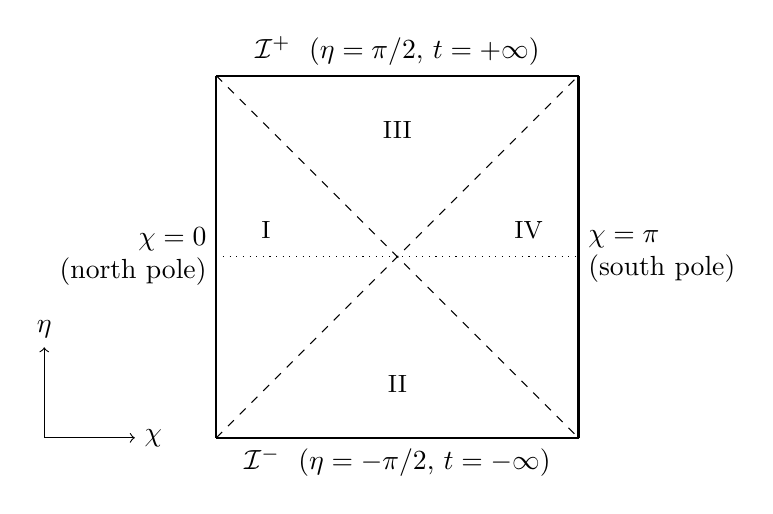
\begin{tikzpicture}[scale=1.15]
  \def\s{4}
  % square
  \draw[thick] (0,0) -- (\s,0);
  \draw[thick] (0,\s) -- (\s,\s);
  \draw[thick] (0,0) -- (0,\s);
  \draw[thick] (\s,0) -- (\s,\s);
  % horizons of observer at chi=0
  \draw[dashed] (0,\s) -- (\s,0);
  \draw[dashed] (0,0) -- (\s,\s);
  % labels
  \node[above] at (\s/2,\s) {$\mathcal{I}^+$ \ ($\eta=\pi/2$, $t=+\infty$)};
  \node[below] at (\s/2,0) {$\mathcal{I}^-$ \ ($\eta=-\pi/2$, $t=-\infty$)};
  \node[left, align=right] at (0,\s/2) {$\chi=0$\\(north pole)};
  \node[right, align=left] at (\s,\s/2) {$\chi=\pi$\\(south pole)};
  \node at (0.55,\s/2+0.3) {\small I};
  \node at (\s/2,0.6) {\small II};
  \node at (\s/2,\s-0.6) {\small III};
  \node at (\s-0.55,\s/2+0.3) {\small IV};
  % throat
  \draw[dotted] (0,\s/2) -- (\s,\s/2);
  % axes
  \draw[->] (-1.9,0) -- (-1.9,1.0) node[above] {$\eta$};
  \draw[->] (-1.9,0) -- (-0.9,0) node[right] {$\chi$};
\end{tikzpicture}
\end{center}

Features of the diagram:
\begin{itemize}
\item Each interior point represents a two-sphere of radius $\propto\sin\chi$. The left and right vertical edges, $\chi=0$ and $\chi=\pi$, are the north and south poles of the $S^3$, where this sphere shrinks to zero size. They are regular points, not boundaries of spacetime.
\item The top and bottom edges, $\eta=\pm\pi/2$ ($t=\pm\infty$), are future and past (timelike and null) infinity $\mathcal{I}^\pm$. In de Sitter these are \emph{spacelike} surfaces, unlike Minkowski space, where null infinity is null.
\item The dashed diagonals are null rays. A light ray leaving the north pole at $\eta=-\pi/2$ only just reaches the south pole at $\eta=+\pi/2$, so no single observer can ever see the whole spacetime. For an observer at $\chi=0$, the line from $(\chi,\eta)=(\pi,-\pi/2)$ to $(0,\pi/2)$ is their \textbf{future event horizon}: events above and to the right of it (III, IV) can never send signals to the observer. The line from $(0,-\pi/2)$ to $(\pi,\pi/2)$ is their \textbf{past (particle) horizon}: events below and to the right of it (II, IV) can never be influenced by them. Region I (the ``static patch'') is the only part of the spacetime in causal contact with the observer in both directions. Region IV is the static patch of the antipodal observer.
\item The dotted line $\eta=0$ ($t=0$) is the throat of minimum size $a=L$, where contraction turns into expansion.
\end{itemize}

%==========================================================
\ques{6}

\qpart{a} Under an infinitesimal diffeomorphism $x^\mu\to x^\mu+\xi^\mu$, $h_{\mu\nu}\to h_{\mu\nu}+\partial_\mu\xi_\nu + \partial_\nu\xi_\mu$. Since $h\to h+2\partial\cdot\xi$,
\be
\bh_{\mu\nu}\to \bh_{\mu\nu} + \partial_\mu\xi_\nu + \partial_\nu\xi_\mu - \eta_{\mu\nu}\partial^\rho\xi_\rho
\quad\Rightarrow\quad
\partial^\mu\bh_{\mu\nu}\to\partial^\mu\bh_{\mu\nu} + \partial^\mu\partial_\mu \xi_\nu \,.
\ee
Choosing $\xi_\nu$ to solve $\Box\xi_\nu = -\partial^\mu\bh_{\mu\nu}$, which is always possible, imposes the \textbf{Lorenz (de Donder/harmonic) gauge}
\be
\partial^\mu\bh_{\mu\nu} = 0 \,.
\ee
In this gauge the second term, $\partial^\rho\partial_{(\mu}\bh_{\nu)\rho} = \tfrac12\left(\partial_\mu\partial^\rho\bh_{\nu\rho}+\partial_\nu\partial^\rho\bh_{\mu\rho}\right)$, and the third term, $\propto\partial^\rho\partial^\sigma\bh_{\rho\sigma}$, both vanish. The linearised Einstein equation becomes
\be
\Box\bh_{\mu\nu} = -16\pi G\,T_{\mu\nu} \,,\qquad \Box = \partial^\rho\partial_\rho = -\partial_t^2 + \nabla^2 \,.
\ee
In vacuum, $T_{\mu\nu}=0$, this is the \textbf{wave equation}, $\left(-\partial_t^2+\nabla^2\right)\bh_{\mu\nu}=0$. Its solutions are disturbances of the metric that propagate at the speed of light, i.e.\ \emph{gravitational waves}. Plane-wave solutions are $\bh_{\mu\nu}=C_{\mu\nu}e^{ik_\rho x^\rho}$ with $k^\mu k_\mu=0$ (null wavevector) and $k^\mu C_{\mu\nu}=0$ (transverse, from the gauge condition). The residual gauge freedom with $\Box\xi_\mu=0$ can be used to go to transverse-traceless (TT) gauge, $h_{0\mu}=0$, $h^\mu{}_\mu=0$, $\partial^i h_{ij}=0$ (so $\bh=h$). This leaves two physical polarisations, $h_+$ and $h_\times$, such as the wave given in part b).

\qpart{b} The metric is $g_{\mu\nu} = \eta_{\mu\nu}+h_{\mu\nu}$:
\be
ds^2 = -dt^2 + \left(1+h_+(t-z)\right)dx^2 + \left(1-h_+(t-z)\right)dy^2 + dz^2 \,.
\ee
This perturbation is in TT gauge: $h_{0\mu}=0$, it is traceless, and it is transverse because it depends only on $t-z$ and has no $z$ components.

\emph{Test particles stay at fixed coordinates.} Consider a particle at rest, $x^\mu(\tau) = (\tau, x_0^i)$, so $\dot x^\mu = (1,0,0,0)$. The geodesic equation gives
\be
\frac{d^2x^i}{d\tau^2} = -\Gamma^i_{00} = -\frac{1}{2}\eta^{ij}\left(2\partial_0 h_{j0} - \partial_j h_{00}\right) = 0 \,,
\ee
because $h_{0\mu}=0$. Likewise $\Gamma^0_{00} = -\frac12\left(2\partial_0h_{00}-\partial_0h_{00}\right)=0$. So freely falling particles initially at rest remain at constant spatial coordinates while the wave passes, with $\tau=t$ to first order. The particles stay at $(0,0,0)$, $(L_x,0,0)$ and $(0,L_y,0)$. The physical effect of the wave is in the proper distance between them.

\emph{Particles along $x$.} At fixed $t$, along the straight line joining them ($y=z=0$, $dt=dy=dz=0$):
\be
ds^2 = \left(1+h_+(t-0)\right)dx^2 \,.
\ee
Since $z=0$ all along the path, $h_+$ is evaluated at $t$ and does not depend on $x$, so
\be
\Delta s = \int_0^{L_x}\sqrt{1+h_+(t)}\,dx = L_x\sqrt{1+h_+(t)} \approx L_x\left(1+\frac{1}{2}h_+(t)\right) \,,
\ee
using $\sqrt{1+\epsilon}\approx 1+\epsilon/2$ for $|h_+|\ll 1$, consistent with linearised theory.

\emph{Particles along $y$.} Similarly, along $x=z=0$ at fixed $t$, $ds^2 = \left(1-h_+(t)\right)dy^2$, so
\be
\Delta s = \int_0^{L_y}\sqrt{1-h_+(t)}\,dy = L_y\sqrt{1-h_+(t)} \approx L_y\left(1-\frac{1}{2}h_+(t)\right) \,.
\ee
When the $x$-separation stretches, the $y$-separation shrinks by the same fraction, and vice versa. This is the characteristic ``$+$'' pattern of the plus polarisation.

\qpart{c}
\textbf{What happens to the binary.} Two compact bodies (black holes or neutron stars) with masses $m_1,m_2$ in a circular orbit have a time-varying mass quadrupole moment, so they radiate gravitational waves. The quadrupole formula gives a radiated power
$P = \frac{32}{5}\frac{G^4}{c^5}\frac{(m_1m_2)^2(m_1+m_2)}{a^5}$ for separation $a$. The waves carry away energy and angular momentum, so the orbital energy $E=-Gm_1m_2/(2a)$ decreases and the orbit shrinks. By Kepler's law, $\omega_{\rm orb}^2 = G(m_1+m_2)/a^3$, so the orbital frequency increases. The waves are emitted at twice the orbital frequency, $f_{\rm GW}=2f_{\rm orb}$, because the quadrupole returns to itself after half an orbit. Their amplitude grows as the bodies speed up and get closer, $h\sim (G\mathcal{M})^{5/3}(\pi f)^{2/3}/(c^4 r)$. The process runs away: the faster the bodies orbit, the more they radiate. This produces a \textbf{``chirp''}, a signal that increases in both frequency and amplitude. The signal has three phases:
\begin{enumerate}
\item \textbf{Inspiral:} a long, slow, quasi-circular phase in which the separation decreases adiabatically. The signal is a nearly sinusoidal wave whose frequency and amplitude increase slowly, then faster and faster. It is well described by post-Newtonian theory. The rate of frequency change depends on the masses mainly through the \emph{chirp mass}, $\dot f = \frac{96}{5}\pi^{8/3}\left(\frac{G\mathcal{M}}{c^3}\right)^{5/3} f^{11/3}$ with $\mathcal{M} = (m_1m_2)^{3/5}/(m_1+m_2)^{1/5}$, so measuring $f$ and $\dot f$ gives $\mathcal{M}$.
\item \textbf{Merger:} once the separation reaches a few times $G(m_1+m_2)/c^2$ (around the innermost stable circular orbit), the bodies plunge together and their horizons merge into a single, highly distorted black hole. This is the strong-field, highly nonlinear regime, computed with numerical relativity. The signal reaches its maximum amplitude and frequency here, with peak frequency $\sim c^3/(G M_{\rm tot})$.
\item \textbf{Ringdown:} the distorted remnant settles down to a stationary Kerr black hole by radiating away its deformations in \emph{quasinormal modes}. The signal is an exponentially damped sinusoid, $h\propto e^{-t/\tau}\cos(\omega_{\rm QNM}t+\phi)$. By the no-hair theorem, $\omega_{\rm QNM}$ and $\tau$ are set only by the final mass and spin, both of order $GM_f/c^3$. The final mass is less than $m_1+m_2$. The difference, a few per cent of the total, is the energy carried away in gravitational waves (about $3M_\odot c^2$ for GW150914).
\end{enumerate}

\textbf{Sketch of the observed signal (strain $h(t)$ at the detector):}
\begin{center}
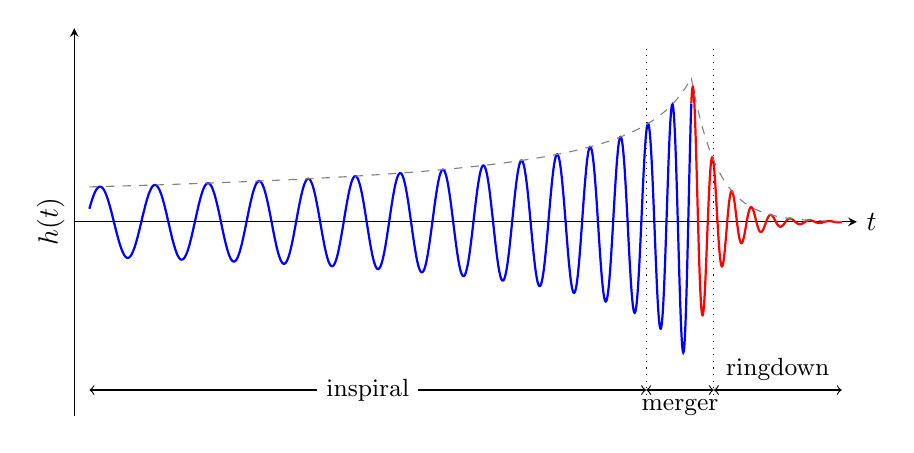
\begin{tikzpicture}
\begin{axis}[
    width=0.95\textwidth, height=6.5cm,
    xmin=-8.2, xmax=2.2, ymin=-1.9, ymax=1.9,
    axis x line=middle, axis y line=left, xlabel={$t$}, ylabel={$h(t)$},
    xlabel style={at={(ticklabel* cs:1)}, anchor=west},
    ticks=none, clip=false]
  % inspiral: A ~ (tc - t)^(-1/2) (schematic), phase ~ (tc-t)^(5/8)
  \addplot[blue, thick, samples=1500, domain=-8:0]
     {(-x+0.5)^(-0.5)*cos(deg(-30*(-x+0.5)^(0.625)))};
  % ringdown: damped sinusoid matched at t=0
  \addplot[red, thick, samples=600, domain=0:2]
     {(0.5)^(-0.5)*exp(-x/0.35)*cos(deg(-30*(0.5)^(0.625) + 24.3*x))};
  % envelope
  \addplot[gray, dashed, samples=200, domain=-8:0] {(-x+0.5)^(-0.5)};
  \addplot[gray, dashed, samples=200, domain=0:2] {(0.5)^(-0.5)*exp(-x/0.35)};
  % phase labels
  \draw[<->] (axis cs:-8,-1.65) -- (axis cs:-0.6,-1.65) node[midway, fill=white] {\small inspiral};
  \draw[<->] (axis cs:-0.6,-1.65) -- (axis cs:0.3,-1.65);
  \node[below] at (axis cs:-0.15,-1.65) {\small merger};
  \draw[<->] (axis cs:0.3,-1.65) -- (axis cs:2,-1.65) node[midway, above] {\small ringdown};
  \draw[dotted] (axis cs:-0.6,-1.7) -- (axis cs:-0.6,1.7);
  \draw[dotted] (axis cs:0.3,-1.7) -- (axis cs:0.3,1.7);
\end{axis}
\end{tikzpicture}
\end{center}
\emph{Schematic:} the inspiral (blue) has slowly increasing frequency and amplitude, the chirp. The amplitude peaks at merger. The ringdown (red) is a rapidly decaying sinusoid at the quasinormal-mode frequency. The gray dashed curve is the envelope. In frequency, the signal sweeps up through the LIGO band ($\sim 10$\,Hz--kHz) in a fraction of a second for stellar-mass black holes.

\textbf{How the interferometer detects the wave.} LIGO is a Michelson interferometer. A laser beam is split at a beam splitter and sent down two perpendicular arms of length $L = 4$\,km, along $x$ and $y$. The end mirrors (test masses) are suspended as pendula, so for horizontal motion at the frequencies of interest they behave as \emph{freely falling test particles}, exactly as in part b). The light reflects back and recombines at the beam splitter. For a $+$-polarised wave travelling perpendicular to the detector plane (along $z$), part b) shows that the proper lengths of the arms change in antiphase:
\be
L_x \to L\left(1+\tfrac12 h_+(t)\right),\qquad L_y\to L\left(1-\tfrac12 h_+(t)\right),\qquad \frac{\Delta(L_x-L_y)}{L} = h_+(t) \,.
\ee
The round-trip light travel times in the two arms therefore differ by $\Delta T\approx 2Lh_+/c$. This shifts the relative phase of the recombined beams by $\Delta\phi\approx 4\pi L h_+/\lambda_{\rm laser}$ and changes the interference pattern. The interferometer is operated near a dark fringe, so a wave produces a light signal at the photodetector proportional to $h_+(t)$. In general the output is $h(t)=F_+h_+ + F_\times h_\times$, with antenna pattern factors depending on the source direction. The detector thus records the waveform $h(t)$ sketched above directly. Typical strains are $h\sim 10^{-21}$, corresponding to arm-length changes $\Delta L\sim 10^{-18}$\,m, far smaller than a proton. Fabry--P\'erot arm cavities (which make the light bounce many times and lengthen the effective arm length), power recycling, seismic isolation, and coincidence between widely separated detectors (Hanford, Livingston, Virgo) make the measurement possible.

\textbf{Connecting the signal to the binary.}
\begin{itemize}
\item The frequency of the wave is twice the orbital frequency. The chirp, increasing frequency and amplitude, is the direct signature of the orbit shrinking as energy is radiated away.
\item The rate of the chirp ($f$ and $\dot f$ during the inspiral) gives the chirp mass $\mathcal M$. Higher-order corrections to the phase give the mass ratio and spins.
\item The frequency at which the inspiral ends and the merger peak occurs scales as $1/M_{\rm tot}$: heavier binaries merge at lower frequency.
\item The ringdown frequency and damping time give the mass and spin of the final Kerr black hole, testing the no-hair theorem. Comparing $M_f$ with $m_1+m_2$ gives the energy radiated.
\item Since $h\propto 1/r$, the amplitude combined with the masses (known from the phase evolution) gives the luminosity distance to the source (``standard siren'').
\end{itemize}

\end{document}
